\subsection{Backpropagation in feedforward multi-layer networks}

All training algorithms were tested using a FFNN with 5 neurons in the hidden layer and 1 neuron in the output layer with different epochs. Two main experiments were executed on a free-noisy data and a noisy data. Due to space constraint, only results on noisy data are shown in \ref{noisy_section2}.

%\begin{figure}[!htbp]
%\caption{Results of the FFNN prediction using different training algorithms in a free-noisy data.}
%\label{pure_section2}
%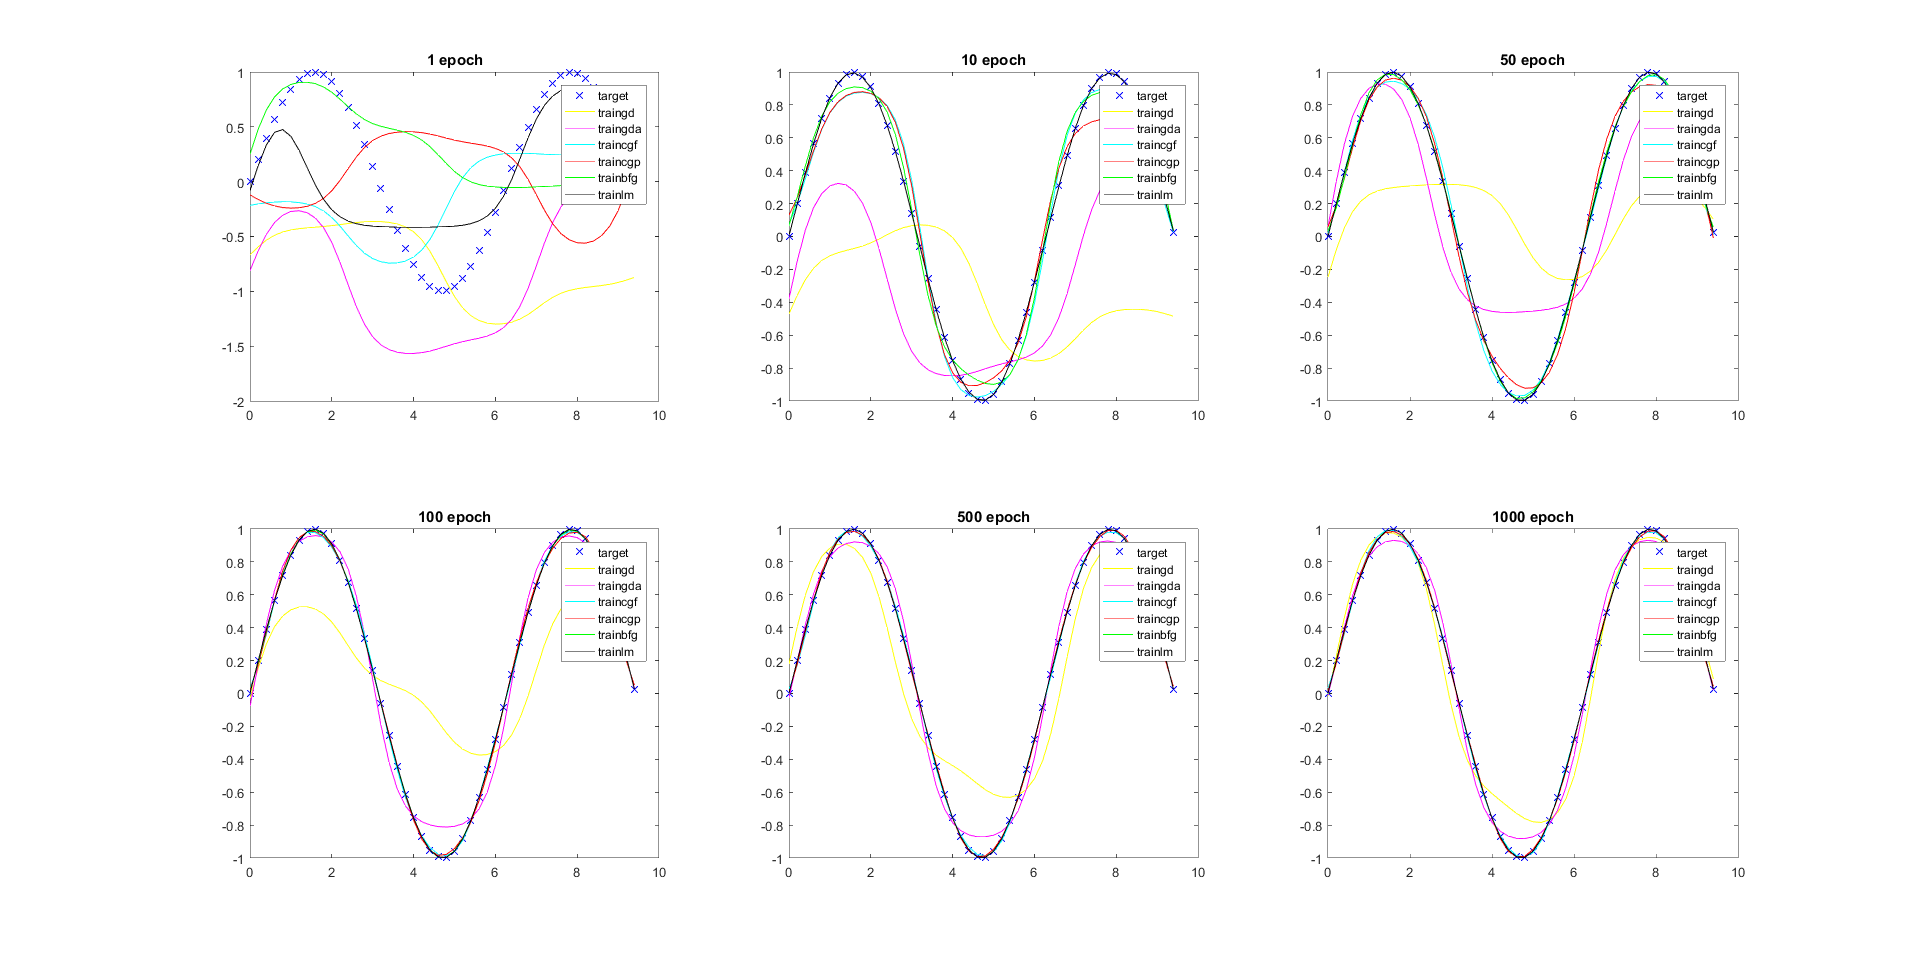
\includegraphics[width=\textwidth]{figures_1/pure_section2}
%\centering
%\end{figure}
\bigbreak
The results clearly indicate that \textit{Levenberg-Marquardt} algorithm (trainlm) converges quicker than the other learning algorithms. As we expected, \textit{Gradient descent} algorithm (traingd) is the slowest to converge. One interesting point in figure \ref{noisy_section2} is that \textit{trainlm} tends to overfit the curve, which illustrate that one should consider an early stop criteria before \textit{trainlm} starts to overfit in order to increase the generalization of the overall model.

\begin{figure}[!htbp]
\caption{Results of the FFNN prediction using different training algorithms in a noisy data.}
\label{noisy_section2}
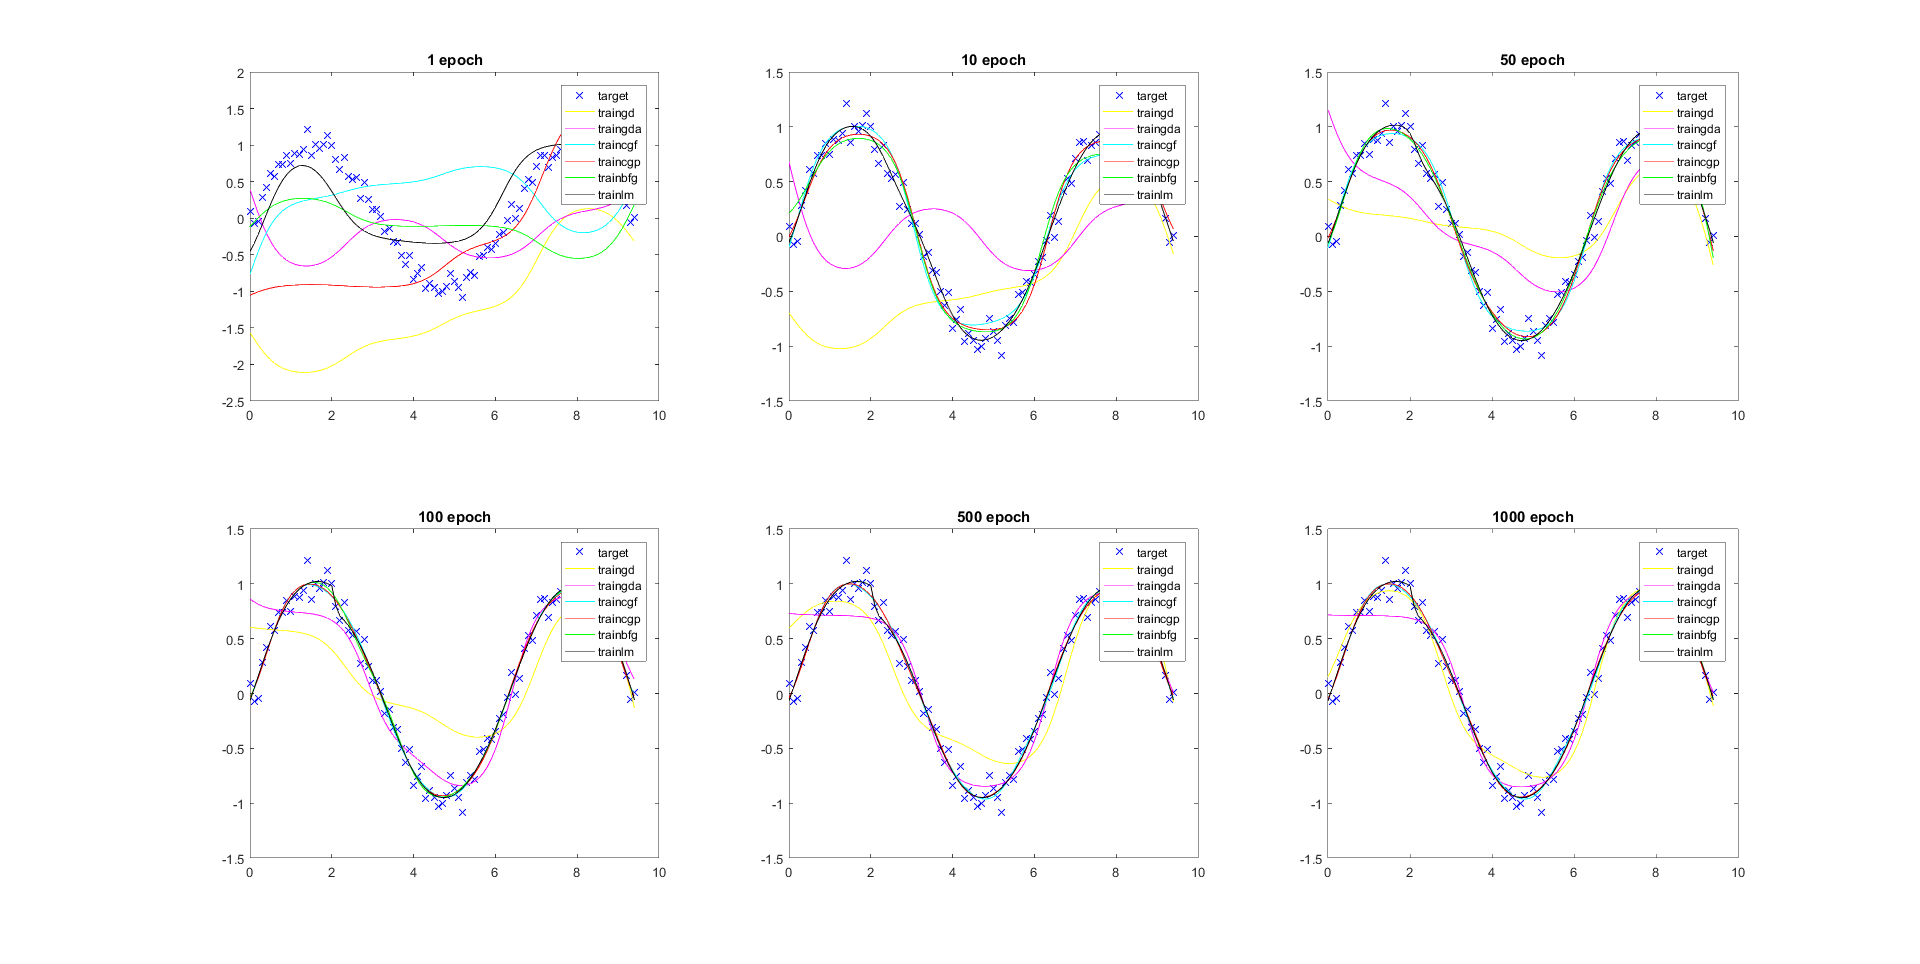
\includegraphics[width=\textwidth]{figures_1/noisy_section2}
\centering
\end{figure}


\subsection{Bayesian inference of networks hyperparameters}
\textit{Bayesian regularization backpropagation} algorithm (trainbr) was tested on a noisy data, similar to the previous section, as well as \textit{trainlm}. Different numbers of neurons were tested. Figures \ref{noisy_section24} and \ref{noisy_section25} show the extreme results of the experiments.
\bigbreak
It it is shown that, at the beginning of the learning phase,  \textit{trainbr} has a very bad model compared to \textit{trainlm}. However after a relatively small number of epochs \textit{trainbr} converges. According with the experiments, the speed rate to obtain a fairly good model from the \textit{trainbr} is pretty similar to \textit{trainlm}. The number of neurons in the hidden layer clearly affect both algorithms. The bigger the number of neurons has, the bigger the overfitting is; which implies that the generalization of the model is small. To conclude, a good trade-off between number of neurons and epochs must be set properly in order to have a good model with high generalization.
\begin{figure}[!htbp]
\caption{Results of the FFNN prediction using \textit{Bayesian regularization backpropagation} and \textit{Levenberg-Marquardt} algorithms in a noisy data using 5 neurons in the hidden layer.}
\label{noisy_section24}
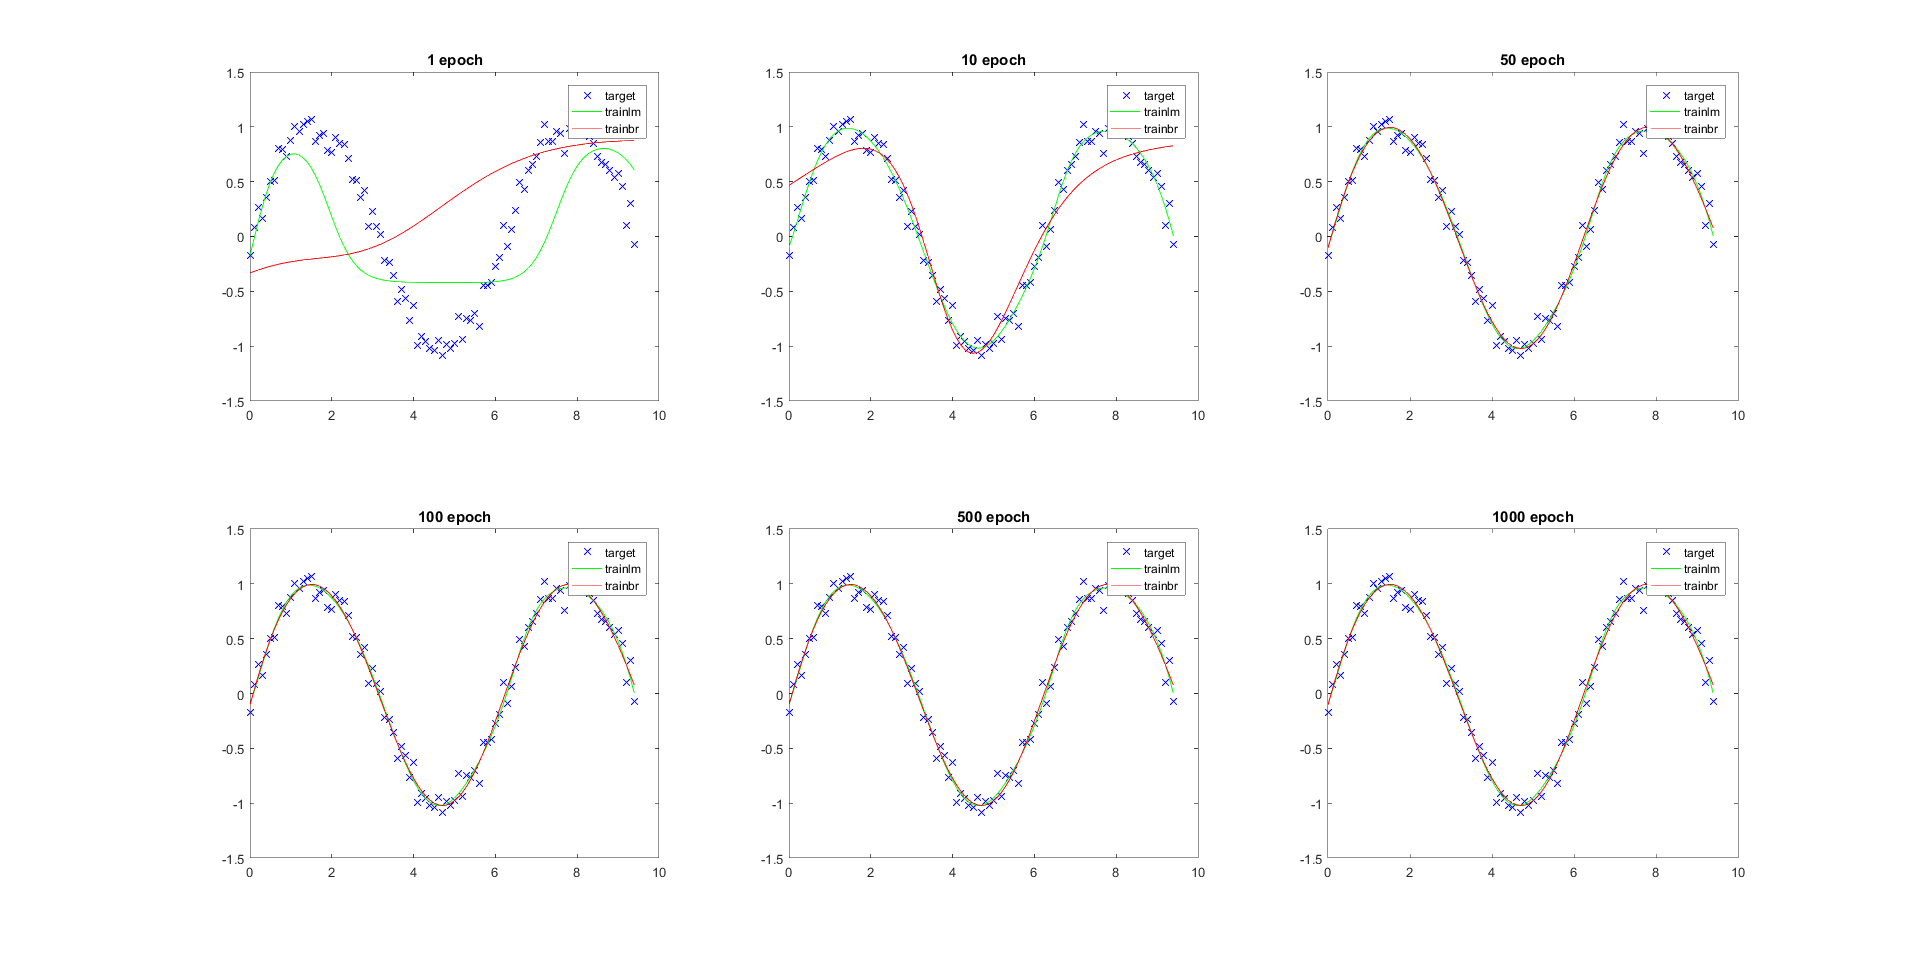
\includegraphics[width=\textwidth]{figures_1/noisy_section4_5n}
\centering
\end{figure}

\begin{figure}[!htbp]
\caption{Results of the FFNN prediction using \textit{Bayesian regularization backpropagation} and \textit{Levenberg-Marquardt} algorithms in a noisy data using 30 neurons in the hidden layer}
\label{noisy_section25}
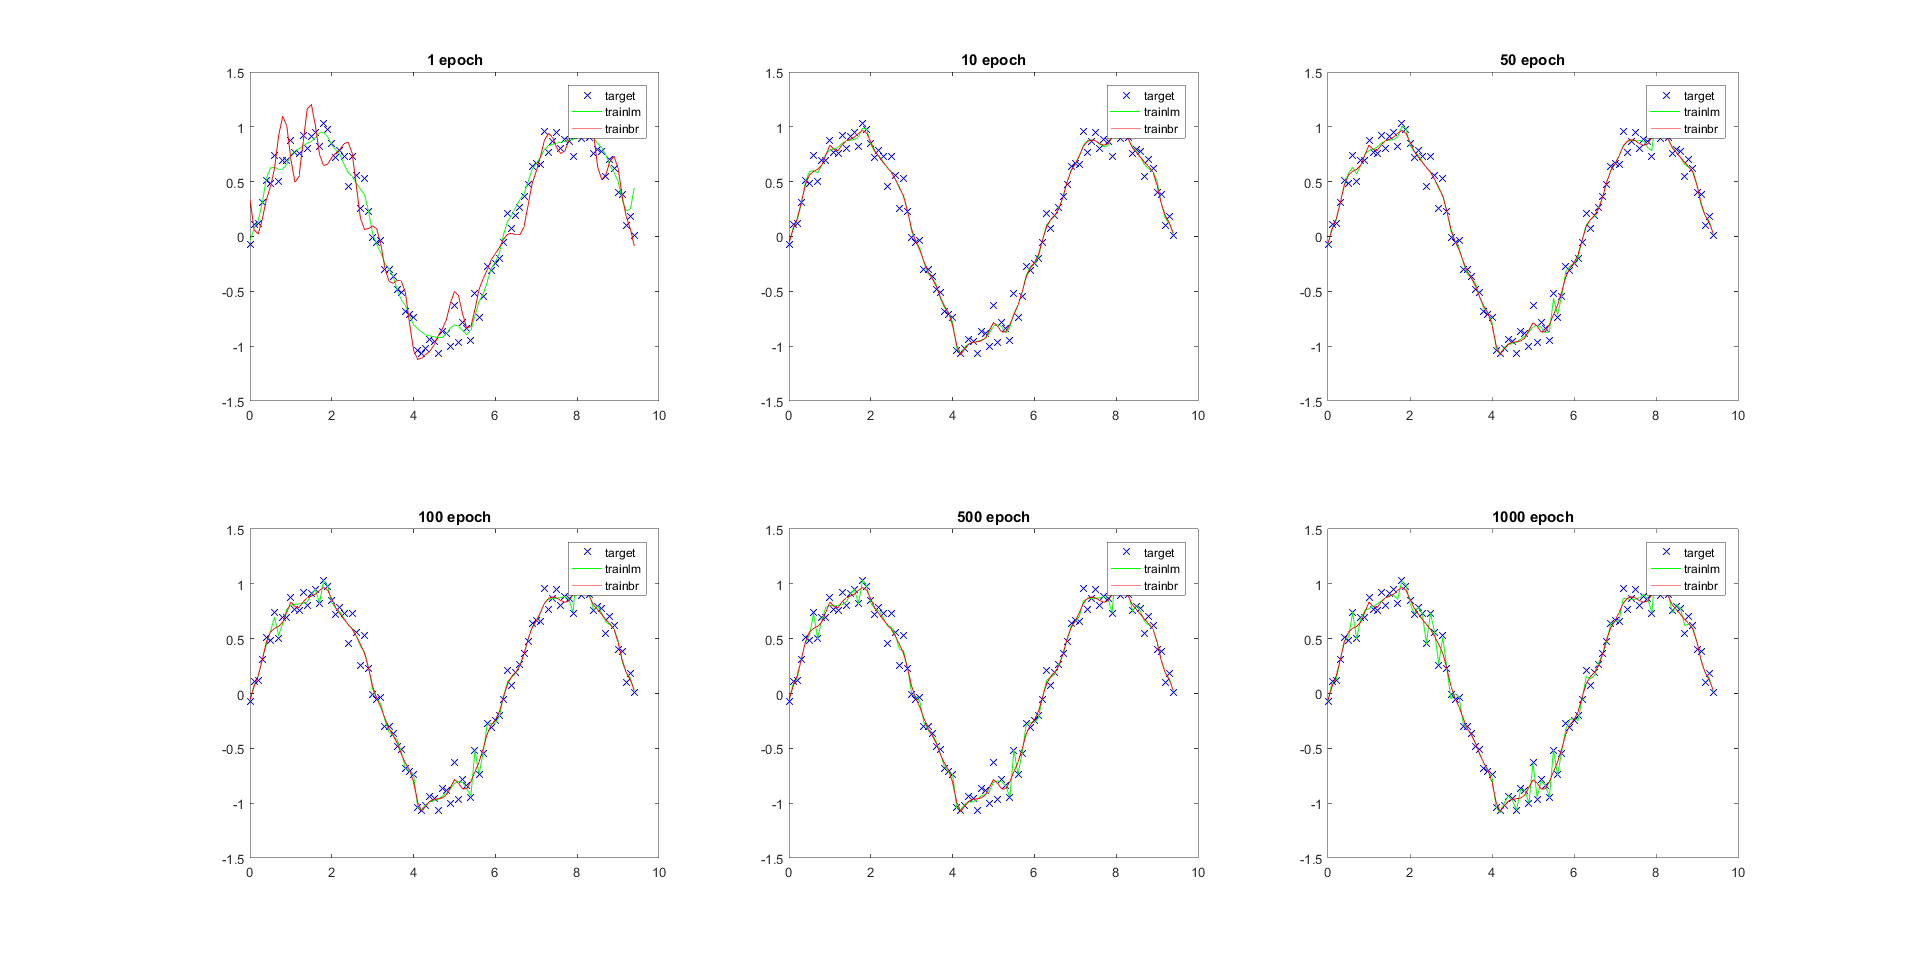
\includegraphics[width=\textwidth]{figures_1/noisy_section4_30n}
\centering
\end{figure}